\lfoot{Autor: Faiku Fitim}
\subsection{Android App}

Die Android App wurde mittels Java erstellt wobei als Programmieroberfläche Android Studio verwendet wurde.
Für jede Klasse wurde ein XML Layout als View generiert, wodurch eine Verbindung zwischen Code und Layout geschaffen wurde.

\subsubsection{Code-Dokumetation}
\lstinputlisting[caption=Design-Beispiel, style=javastyle]{code/MyActivity.java}
 Um die Grafiken bestmöglich darzustellen und dabei eine möglichst hohe Anzahl an Usern zu erreichen, entschieden wir uns eine Android App zu entwickeln.
 Dabei achteten wir besonders auf die Benutzerfreundlichkeit der Applikation.
 Die wichtigsten Kriterien waren, dass der Fahrer im Straßenverkehr nicht abgelenkt wird, er sehr leicht zwischen den einzelnen Features wechseln kann und die Informationen intuitiv aufbereitet sind.
 
 Um die App zu realisieren erstellten wir mehrere Fragments zwischen denen man hin und her \textit{swipen} kann.
 

 Es wurde zuerst eine MainActivity Klasse erstellt, welche von FragementActivity erbt und von ActionTabListener implementiert, um die Methoden onTabReselected, onTabselected und onTabunselected zu überschreiben.   
 
            
Im Anschluss setzten wir die View der Klasse auf main durch:  

\lstinputlisting[firstline=1,lastline=1, style=javastyle]{code/examples.java}

Wir erstellten ein Objekt von ActionBar und fügten mehrere Tabs hinzu und setzten das Layout für die Navigation der Tabs mittels:

\lstinputlisting[firstline=2,lastline=2, style=javastyle]{code/examples.java}

Anschließend wurden mehrere Tabs hinzugefügt mit der Methode:

\lstinputlisting[linerange={4-8}, style=javastyle]{code/examples.java}


Nun gehen wir über zu unserem Design unter main.xml
\lstinputlisting[caption=Design main, style=xmlstyle]{code/main.xml}
Es wurde ein ViewPager Layout erstellt welches das \textit{swipen} möglich macht:

\lstinputlisting[firstline=10,lastline=10, style=xmlstyle]{code/examples.java}

Wir übergeben dem Layout ebenfalls eine ID auf die wir von unserer main Activity aus zugreifen: 
\lstinputlisting[firstline=12,lastline=12, style=xmlstyle]{code/examples.java}



Nun erstellen wir eine Fragementadapter-Klasse um die einzelnen Tabs den Klassen zuzuteilen. 
Die Klasse hat einen Konstruktor, welcher von der Superklasse das FragementManager Objekt übergeben bekommt.
Weiters hat die Klasse eine getItem Methode mit dem Input eines int Wertes. 
\lstinputlisting[caption=PageAdapter, style=javastyle]{code/FragementPageAdapter.java}


Es wird hierbei überprüft ob, welcher Tab aktiviert wurde, und der wird der entsprechenden Klasse eingeteilt. 
Sie hat noch eine getCount() Methode, welche die Anzahl der Tabs zurückgibt in unserem Fall 3.


Wir erstellen auf der Main Klasse zwei Objekte, nämlich:
\lstinputlisting[linerange={14-18}, style=javastyle]{code/examples.java}

Dies wird gemacht um zwischen den Oberflächen wechseln zu können.

 

\subsubsection*{Implementierung von MPAndroidChart}
Als nächstes haben wir mithilfe der MPAndroidchart Library einige Graphen erstellt und sie mit Daten befüllt.

\lstinputlisting[caption=Liniendiagramm Beispiel, style=javastyle]{code/Beschleunigungskraefte.java}

<<<<<<< HEAD

 

\begin{wrapfigure}{r}{0.6\textwidth}
	\centering
	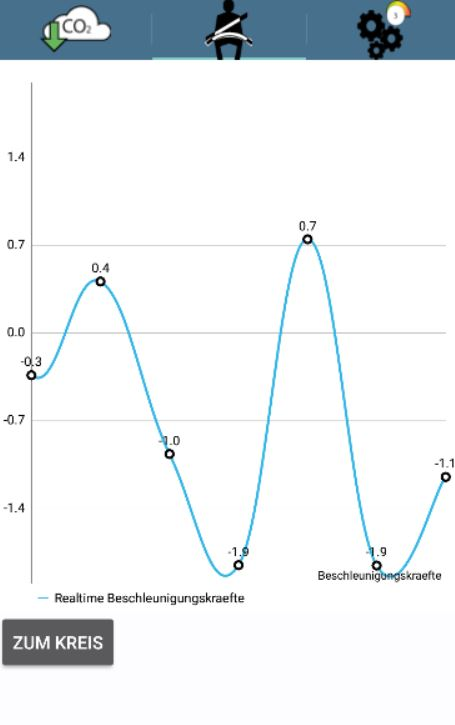
\includegraphics[width=0.5\textwidth]{images/Liniendiagramm}
	\caption{Beschleunigungskräfte Längstrichtung }
\end{wrapfigure}




=======
>>>>>>> 4b305ee98c8a6cb99d86a6a2443ec5617cf8319b
\clearpage % DO NOT REMOVE